%  Created by QING Pei on 2012-02-10
%  Copyright (c) 2012 QING Pei, edwardtoday@gmail.com. All rights reserved.
%
%  Mobile Data Management of Location-dependent Information Services - A Survey
%  COMP5527 Assignment 1, PolyU, HK

% \documentclass{acm_proc_article-sp}
\documentclass[12pt,a4paper]{article}
\usepackage{graphicx}
\begin{document}

% \title{Location-Based Services and Data Management - A Survey\titlenote{COMP 5527 Mobile Computing and Data Management Assignment One}}
\title{Location-Based Services and Data Management - A Survey\footnote{COMP 5527 Mobile Computing and Data Management Assignment One}}
\author{QING Pei, 11500811G}
\date{\today}
% \subtitle{\today}
% 
% \numberofauthors{1}
% \author{
% \alignauthor QING Pei 11500811G\\
% \affaddr{The Hong Kong Polytechnic University}\\
% \affaddr{Hung Hom Kowloon, Hong Kong}
% \email{pei.qing@connect.polyu.hk}
% }

\maketitle

\begin{abstract}
Location dependent data in mobile computing context requires novel management approaches. The objective of this paper is to provide an overview of location-based services regarding the terms, technologies and standards. How location information is stored, communicated and manipulated is discussed as well a variety of applications of such information.
\end{abstract}

% \keywords{Mobile computing, databases, location dependent data, location-based services}

\section{Introduction} % (fold)
\label{sec:intro}
% overview and organization of this paper
In recent years, mobile computing has attracted a great interest both in the industry and in research. The daily use of mobile devices has thrived magnificently in the past decade. Providing data access on these mobile devices anywhere and any time is an important field of study.

In Section \ref{sec:overview}, a brief introduction of the topic is presented. Following that is Section \ref{sec:challenges} which lists the challenges in the field. Section \ref{sec:existing} describes the current status of research work related to the topic. Finally, conclusions and opportunities for future work is given in Section \ref{sec:conclusions}.
% section intro (end)

\section{Overview of the selected topic} % (fold)
\label{sec:overview}
% tell people what the topic is about and its basic concepts
\subsection{Location-Based Services} % (fold)
\label{sub:location_based_services}
A location-based service (LBS) can be described as an application that is dependent on a certain location. Triggered and user-requested LBS are the two major categories. \cite{DRoza:2003wz}

The range and variance of location services is considerable. The location information can be used by the mobile operator or service provider to determine billing information, such as whether the user is in a home zone or roaming overseas. In addition, emergency services and lawful interception services will want information on a user's location at a specific point of time. \cite{Adams:2003un}

Typical services will include the following:

\begin{itemize}
	\item fleet management
	\item asset management
	\item navigation
	\item virtual sightseeing
	\item searching for nearby bank, restaurant, restroom, etc.
	\item localized mobile Yellow Pages
	\item localized internet radio, weather report, etc.
\end{itemize}
% subsection location_based_services (end)

\subsection{Location Dependent Data} % (fold)
\label{sub:location_dependent_data}
Location dependent data (LDD) refers to data whose values depend on location. A geographic domain is the entire area covered by the mobile computing platform. A location is a precise point within the geographic domain representing the smallest identifiable position in the domain, which can be expressed with a latitude/longitude pair.\cite{Dunham:1998ci}
% subsection location_dependent_data (end)

\subsection{Positioning Technology} % (fold)
\label{sub:positioning_technology}

\subsubsection{Global Positioning System (GPS)} % (fold)
\label{ssub:global_positioning_system_gps_}
The Global Positioning System (GPS) is a space-based satellite navigation system, can provide all-weather location and time information anywhere on or near the Earth, there are four or more GPS satellites unobstructed line of sight. It is by the U.S. government to maintain freedom of access to any GPS receiver. GPS solutions around the world, military, civilian and commercial users to provide key capabilities. In addition, the Global Positioning System is the backbone of the modern global air transport system. \cite{wiki-gps}

In 1973, the GPS project development, to overcome the limitations of the previous navigation system, a combination of ideas from several predecessors, including some confidential project design researches from the 1960s. \cite{national1995global} The creation of GPS and the U.S. Department of Defense (DOD) and 24 satellites in the first run. It began full operation in 1994.

Progress in the technology of existing systems and new requirements have led to efforts to modernize the GPS system and the implementation of next-generation GPS III satellites, and the next generation of operational control system (OCX). \cite{gpsocx} Announcement from the Vice President and the White House in 1998 initiated these changes. 2000, the U.S. Congress authorized the modernization effort, referred to as GPS III.

In addition to GPS, other systems are in use or under development. Only the Russian military in Russia's Global Navigation Satellite System (GLONASS), the civilian population until it is fully available until 2007. Planned European Galileo positioning system, the Beidou navigation system and the Indian Regional Navigation Satellite System.

The principle behind GPS is the measurement distance between the satellite and receiver (or ``area''). Satellite tells us exactly where we by broadcasting data in their orbits, which receivers use to calculate their positions. Its principle is this: If we know our exact distance from the satellite in space, we know that we are somewhere on satellite radius of an imaginary sphere surface distance equal to the radius if we know the exact distance from the two satellites we know our place in the intersection of two areas on the line. And, if we take the third and fourth two more satellite measurements, we can find our place the GPS receiver to handle the satellite measurement of the scope and its location. \cite{gpsprimer}

GPS uses the coordinate system called WGS 84 World Geodetic System 1984. It allows the surveyor around the world to produce all the longitude and latitude lines, locating places and things, the common frame of reference, like you see in the school map. Similarly, the GPS from the U.S. Naval Observatory in Washington, DC, time synchronization, GPS system time, all the elements, like Harrison's astronomical clock is synchronized in the Greenwich Mean Time. Figure \ref{fig:howgpsworks} illustrates the process of global positioning system.

\begin{figure}
\centering
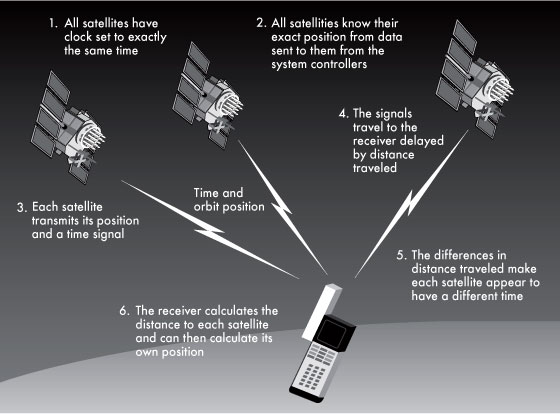
\includegraphics[width=.85\textwidth]{fig/5steps-illustration}
\caption{How GPS Works}
\label{fig:howgpsworks}
\end{figure}

% subsubsection global_positioning_system_gps_ (end)

\subsubsection{Differential GPS (DGPS)} % (fold)
\label{ssub:differential_gps_dgps_}
Differential global positioning system (DGPS) is a global positioning system provides positioning accuracy from 15 meters in the name of the GPS accuracy the best case about 10 cm enhanced. The difference between the differential global positioning system uses a fixed, ground-based reference station network broadcast the location indicated by the satellite systems and the known fixed location. Broadcast satellite pseudorange and the actual pseudo-range (internal calculation) the difference between the receiving station may be caused by the same number of pseudo-range correction. Local shorter distance terrestrial transmitters, digital correction signals are usually broadcast. \cite{wiki-dgps}
% subsubsection differential_gps_dgps_ (end)

\subsubsection{GSM Cellular Location} % (fold)
\label{ssub:gsm_cellular_location}
Due to the nature of the GSM mobile telephone network in cells, it is possible to determine the position of an ordinary GSM mobile phone. Described in The CELLID the basic system is a little rough, but the technology can provide to improve the accuracy. This section describes one of the methods increasing CELLID accuracy, but other countries also exist. GPS cellular localization is much stronger signal, and therefore the operating room, it is by the urban canyon effect (GSM network coverage) and impact. \cite{DRoza:2003wz}

Network-based technologies, the use of the network service provider's infrastructure to determine the location of the mobile phone. Advantage of Network-based technologies (from the perspective of mobile operators), they can achieve non-invasive, does not affect the phone. Based on the accuracy of the network technology, cell recognition is not accurate and triangular, moderately accurate, and new ``link'' the most accurate timing method. Based on the accuracy of the network technology is not only dependent on the concentration of cells at the base station, and the urban environment, to achieve the highest possible precision execution timing. \cite{wiki-cellloc}
% subsubsection gsm_cellular_location (end)

% subsection positioning_technology (end)

\subsection{Representation of Location Information} % (fold)
\label{sub:representation_of_location_information}
Regardless of the methods used to find the return of the original data is usually co-ordination may be wrong parameters. While this is by far the most accurate statements, in the majority of the user's original data is not very useful, can only become valuable when explained in different ways. A position can be described relative to prior known location. As the name of a place known as geocoding points of interests table usually contains the name of the towns and cities, street name or place of business in some applications can also be used to customize the blog. \cite{DRoza:2003wz}

% subsection representation_of_location_information (end)
% section overview (end)

\section{Challenges} % (fold)
\label{sec:challenges}
% Identification and description of main challenging issues and technologies

\subsection{Challenges for Positioning Technology} % (fold)
\label{sub:challenges_for_positioning_technology}

\subsubsection{Drawbacks of GPS} % (fold)
\label{ssub:drawbacks_of_gps}
GPS provides an unprecedented level of positioning accuracy, but it does have some drawbacks. Satellites in high orbit, and broadcast a large area of ​​the signal is very weak. Pseudo-random nature of the small footprint antenna signal allows, but because of the weak signal is received, you need a reasonably unobstructed sky. Repair of the trees in the next position in the GPS receiver cannot obtain a building coverage, and even limit the high-rise buildings of the sky. \cite{DRoza:2003wz}
% subsubsection drawbacks_of_gps (end)

\subsubsection{Cellular Location Limitations} % (fold)
\label{ssub:cellular_location_limitations}
Based on one of the main challenges of the network technology, is to work in close cooperation with the ISP, because it requires the operators of infrastructure hardware and software installation. Under normal circumstances, such as the legislative framework for the E911, will be in place to force the cooperation of the ISP, as well as to maintain the privacy of information. \cite{wiki-cellloc}
% subsubsection cellular_location_limitations (end)

% subsection challenges_for_positioning_technology (end)

\subsection{Challenges on Mobile Devices} % (fold)
\label{sub:challenges_on_mobile_devices}
In whatever cases, LDD or LBS has to be processed or consumed by mobile devices. Limitations of the device itself also pose challenges for providing a good service. Some of the shortcomings of mobile devices compared to fixed ones are:

\begin{itemize}
	\item intermittent connectivity
	\item short battery life
	\item slow data transmission
	\item limited memory size
	\item limited storage size
	\item weak processing unit
	\item small display size
\end{itemize}

And due to the fact that mobile devices have limit power, the early generations of mobile resources are not compatible with the general purpose protocols such as the standard HTTP.
% subsection challenges_on_mobile_devices (end)

\subsection{Challenges for Query Processing} % (fold)
\label{sub:challenges_for_query_processing}
The major difficulties for query processing of location dependent data is that the location is frequently updated and that the position information is often not accurate to some extent when using some of the positioning technology mentioned in \ref{sub:positioning_technology}.
% subsection challenges_for_query_processing (end)

% section challenges (end)

\section{Existing work} % (fold)
\label{sec:existing}
% Review of existing works with classifications and discussions

\subsection{Adapting Existing Techniques to Mobile Environment} % (fold)
\label{sub:adapting_existing_techniques_to_mobile_environment}
As mentioned in \ref{sub:challenges_on_mobile_devices}, limitations of mobile devices make existing computing techniques no longer efficient or appropriate. Under this circumstance, a lot work has been done to adapt the existing techniques to the mobile environment. \cite{imielinski1993data,imielinski1996introduction,pitoura1998data,jing1999client,ISI:000079296600012}
% subsection adapting_existing_techniques_to_mobile_environment (end)

\subsection{Location Dependent Data} % (fold)
\label{sub:location_dependent_data_c}
Prasad et al. propose a data model for representing moving objects in database systems. It is called the Moving Objects Spatio-Temporal (MOST) data model. Future Temporal Logic (FTL) is proposed as the query language for the MOST model, and devise an algorithm for processing FTL queries in MOST. \cite{prasad1997modeling} The concept dynamic attributes whose value change continually as a function of time is introduced as well.Both spatial and temporal aspects into the location dependent processing are incorporated in their approach.

The approach of Dunham et al. for dealing with LDD queries and transactions is quite different from that of the MOST approach. They don't require that specific location data be  placed in the database (although this would be allowed with their approach). The database can be thought of as partitioned into locations. Each partition would have the correct data values for that location. Their work does not actually conflict with that in \cite{prasad1997modeling}. LDD could be partitioned using their approach and could follow the MOST approach as well. \cite{Dunham:1998ci} Figure \ref{fig:dunham_ldd} shows their proposed approach to implement location dependent data. 

A Mobile Unit (MU) requests a query. It then is routed to the mobile service switching center (MSC) to determine the correct service control point (SCP), the news service. Each MSC has a unique SCP for each ISP. SCP has a database containing the location of the relevant data. Space-time copy of the database access any data continuously from the cells in the MSC area. It also contains a copy of the space of those objects in the MSC area, the area with household data. There is network connectivity to all SCPS, Appropriate distributed database concurrency control, across, the SCPS, as well as the recovery method. If the data are too large to be stored in the SCP, you can add the appropriate database server on the fixed network. In this case, the SCP query routing process server assumes that the requirements of the position to add the default location binding, so that has been determined, and receive a message when the SCP MSC. If the query contains another location, then this will override the default location and SCP forwards queries deal with the location. \cite{Dunham:1998ci}

\begin{figure}
\centering
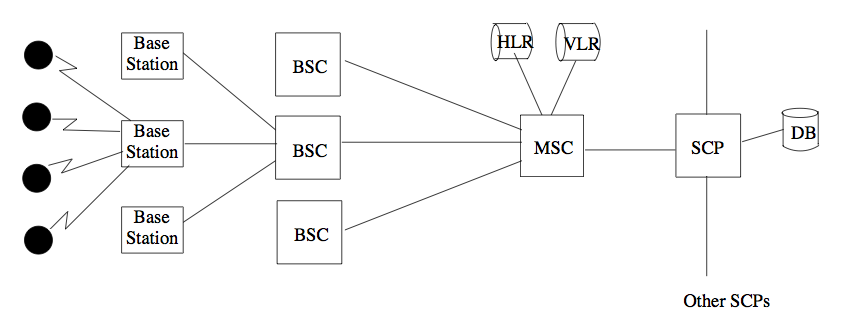
\includegraphics[width=.85\textwidth]{fig/Dunham_LDD}
\caption{Dunham et al.'s Implementation Architecture for LDD}
\label{fig:dunham_ldd}
\end{figure}
% subsection location_dependent_data_c (end)

\subsection{Location Representation} % (fold)
\label{sub:location_representation}
For many applications, including fleet management, tracking and routing, the most logical positional representation is graphical. There are many companies that specialize in the provision of map data including The AA \cite{theaa}, Ordnance Survey \cite{ordnance} and Bartholomew \cite{bartholomew}, with the main difference being one purely of aesthetics. A map image is usually composed of a number of layers, where motorways, roads, city labels and county borders will all appear on separate layers. The application provider may choose which layers to include, and will usually opt to only include certain layers at particular zoom levels to avoid clutter. \cite{DRoza:2003wz}

\subsubsection{Data Formats and Standards} % (fold)
\label{ssub:data_formats_and_standards}
\paragraph{XML} % (fold)
\label{par:xml}
Geographic information system (GIS) industry has formed a set of XML to describe the standard recommendations. They solve two types of geographic information - static (such as rivers, mountains, etc.) and dynamic (events, moving objects). Geography Markup Language (GML), the former information is captured, the latter is the exchange from the point of interests (POIX) the exchange of interest-point mark, captured, the navigation Markup Language (NVML) for the tag line, and event information tag SKiCAL. \cite{DRoza:2003wz}

\begin{itemize}
	\item GML \cite{gml}
	\item POIX \cite{poix}
	\item NVML \cite{nvml}
	\item SKiCAL \cite{SKICal}
\end{itemize}

In summary, an application might use a combination of the above XML-based formats. This can be achieved by using XML namespaces. It is also better to do the processing in the application server, which will guarantee sufficient capacity to handle generic XML processing.
% paragraph xml (end)
% subsubsection data_formats_and_standards (end)
% subsection location_representation (end)

\subsection{Query Processing} % (fold)
\label{sub:query_processing}
Querying location dependent information in mobile environment has been as an important research area and most of the work to date has studied dat management issues of mobile objects and their location information. \cite{imielinski1993data} identifies new challenges and investigates their technical significance. New research problems include management of location dependent data, wireless data broadcasting, disconnection management and energy efficient data access. \cite{pitoura1994building} describes the general architecture of the information system and the main considerations of our design. Then, based on these considerations, \cite{pitoura1994building} presents a system support for maintaining the consistency of replicated data and for providing transaction schemas that account for the frequent but predictable disconnections, the mobility, and the vulnerability of the wireless environment. \cite{pitoura2001locating} presents a comprehensive survey of the various approaches to the problem of storing, querying, and updating the location of objects in mobile computing.

\cite{forman1994challenges} points out that many issues to be dealt with stem from three essential properties of mobile computing: communication, mobility, and portability. \cite{Dunham:1995:MCD:219713.219727} views location dependent queries as asking values of data which changes depending on a location. In \cite{Dunham:1998ci} LDD is defined as spatial replicas depending on its geographic domain. \cite{kumar1998defining} also discusses query processing approaches considering location bindings and physical organization.

Seydim et al. give a formalization of location relatedness in queries. \cite{Seydim:2001wk} differentiates location dependence and location awareness and provides thorough examples to support their approach.

\cite{xu2000querying} identifies queries according to their access to location information. In all types mentioned by \cite{xu2000querying}, Location Binding is assumed to be a ``cell id'' binding to the query. Local queries start from the current Base Station to the root while non-local queries are redirected to the corresponding cell and the replies are, in turn, forwarded back to the current cell. Geographically-Clustered and Geographically-Dispersed queries have to be processed in cell basis. Another type, nearest query has to be process from the current cell and the nearest cell to the farthest until satisfied.
% subsection query_processing (end)

\subsection{Moving Object Databases (MOD)} % (fold)
\label{sub:moving_object_databases}
Most research to date not only has concentrated on query processing issues for location databases but also on the MOD. \cite{prasad1997modeling, wolfson1998moving} These works views location dependent applications as MOD applications.

% subsection moving_object_databases (end)
% section existing (end)

\section{Conclusions} % (fold)
\label{sec:conclusions}
% summarize what you have presented and discussed in the paper and any observations and conclusions you want to draw from the paper
A review of the current status in LDD query processing and LBS data management. First, the characteristics of the mobile environment is introduced and clarified with examples of different types of LBS. With that knowledge, a number of challenges are listed and described. Query processing approaches in the mobile context, including MOD ones, are then discussed.

Future research directions in this field may contain some of the following:

\begin{itemize}
	\item Decentralized architecture. Most mobile service architecture nowadays are centralized. Once the controlling node or the database server fail, the whole system fails as well. Distributed (or decentralized) architecture has been increasingly adopted in other applications such as source code management (Git, Mercurial) and file-sharing (BitTorrent). The design and standardization of a decentralized mobile computing architecture would probably help to build a more robust and available service.
	\item Streaming instead of querying. The current centralized solution implies that there exist a database storing all the location information for incoming queries. When a value is requested frequently from many mobile units, various caching techniques are currently used to support this. However, if a new solution can be found similar to the streaming mechanism in video on demand (VOD) applications using some technique like multicasting, the performance may be improved.
	\item Unified testing framework. Most existing researches test the performance of their approaches by simulation rather than in real mobile environments. Different works use different simulation methods with varied properties. In this case, comparison or benchmarking is almost impossible since the testing results come from different environments. A unified testing framework would solve this problem.
\end{itemize}
% section conclusions (end)

\bibliographystyle{acm}
\bibliography{5527_assign1}

% \balancecolumns
\end{document}
